% LIST for appendix:
% - distribution of response lengths
% - moral foundations questionnaire


\section{Basic Rules on the Subreddit ChangeMyView}\label{app:rules}

Below is a summary of the set of rules to participate in discussions on \texttt{/r/ChangeMyView} as described in April 2018. The current rules can be viewed at \url{https://www.reddit.com/r/changemyview/wiki/rules}

\paragraph{Rules for submission of new discussion posts:}
\begin{enumerate}[A]\singlespacing
\item Explain the reasoning behind your view, not just what that view is (500+ characters required).
\item You must personally hold the view and demonstrate that you are open to it changing.
\item Submission titles must adequately sum up your view and include "CMV:" at the beginning.
\item Posts cannot express a neutral stance, carry a risk of personal endangerment, be self-promotional, or discuss this subreddit (visit r/ideasforcmv instead).
\item Only post if you are willing to have a conversation with those who reply to you, and are available to start doing so within 3 hours of posting.
\end{enumerate}

\paragraph{Rules for commenting in existing discussions:}
\begin{enumerate}[1]\singlespacing
\item Direct responses to a CMV post must challenge at least one aspect of OP’s stated view (however minor), or ask a clarifying question.
\item Don't be rude or hostile to other users.
\item Refrain from accusing OP or anyone else of being unwilling to change their view.
\item Award a delta if you've acknowledged a change in your view. Do not use deltas for any other purpose.
\item Comments must contribute meaningfully to the conversation.
\end{enumerate}


\clearpage
\section{Moral Foundations Dictionary}\label{app:cmvdict}
\textit{Sources:}\\
\bibentry{graham2009liberals}, as well as \url{http://www.moralfoundations.org/}
\vspace{.5cm}

\noindent\textit{Note:}\\
Terms with (*) indicate that the word stem rather than the exact word was matched in the open-ended survey responses.
\vspace{.5cm}

\subsubsection*{Care} amity, benefit*, care, caring, compassion*, defen*, empath*, guard*, peace*, preserve, protect*, safe*, secur*, shelter, shield, sympath*, abandon*, abuse*, annihilate*, attack*, brutal*, cruel*, crush*, damag*, destroy, detriment*, endanger*, exploit, exploited, exploiting, exploits, fight*, harm*, hurt*, impair, kill, killed, killer*, killing, kills, ravage, ruin*, spurn, stomp, suffer*, violen*, war, warl*, warring, wars, wound* 

\subsubsection*{Fairness} balance*, constant, egalitar*, equable, equal*, equity, equivalent, evenness, fair, fair-*, fairly, fairmind*, fairness, fairplay, homologous, honest*, impartial*, justice, justifi*, justness, reasonable, reciproc*, rights, tolerant, unbias*, unprejudice*, bias*, bigot*, discriminat*, dishonest, disproportion*, dissociate, exclud*, exclusion, favoritism, inequitable, injust*, preference, prejud*, segregat*, unequal*, unfair*, unjust*, unscrupulous

\subsubsection*{Loyalty} ally, cadre, cliqu*, cohort, collectiv*, communal, commune*, communis*, communit*, comrad*, devot*, familial, families, family, fellow*, group, guild, homeland*, insider, joint, loyal*, member, nation*, patriot*, segregat*, solidarity, together, unison, unite*, abandon*, apostasy, apostate, betray*, deceiv*, deserted, deserter*, deserting, disloyal*, enem*, foreign*, immigra*, imposter, individual*, jilt*, miscreant, renegade, sequester, spy, terroris*, traitor*, treacher*, treason* 

\subsubsection*{Authority} abide, allegian*, authorit*, bourgeoisie, caste*, class, command, complian*, comply, control, defer, defere*, duti*, duty, father*, hierarch*, honor*, law, lawful*, leader*, legal*, loyal*, mother, mothering, motherl*, mothers, obedien*, obey*, order*, permission, permit, position, preserve, rank*, respect, respected, respectful*, respects, revere*, serve, status*, submi*, supremacy, tradition*, venerat*, agitat*, alienate, apostasy, apostate, betray*, defector, defian*, defy*, denounce, deserted, deserter*, deserting, disloyal*, disobe*, disrespect*, dissent*, dissident, heretic*, illegal*, insubordinat*, insurgent, lawless*, mutinous, nonconformist, obstruct, oppose, protest, rebel*, refuse, remonstrate, riot*, sediti*, subver*, traitor*, treacher*, treason*, unfaithful

\subsubsection*{Sanctity} abstemiousness, abstention, abstinen*, austerity, celiba*, chast*, church*, clean*, decen*, holiness, holy, immaculate, innocent, integrity, limpid, maiden, modesty, piety, pious, preserve, pristine, pure*, purity, refined, sacred*, saint*, steril*, unadulterated, upright, virgin, virginal, virginity, virgins, virtuous, wholesome*, adulter*, apostasy, apostate, blemish, contagio*, debase*, debauche*, defile*, deprav*, desecrat*, dirt*, disease*, disgust*, exploit, exploitat*, exploited, exploiting, exploits, filth*, gross, heretic*, impiety, impious, indecen*, intemperate, lax, lewd*, obscen*, pervert, profan*, profligate, promiscu*, prostitut*, repuls*, ruin*, sick*, sin, sinful*, sinned, sinner*, sinning, sins, slut*, stain*, taint*, tarnish*, tramp, trashy, unchaste, unclean*, wanton, whore, wicked*, wretched*

\subsubsection*{General Morality} bad, blameless, canon, character, commendable, correct, decen*, doctrine, ethic*, evil, exemplary, good, goodness, honest*, ideal*, immoral*, indecen*, integrity, laudable, lawful*, legal*, lesson, moral*, noble, offend*, offensive*, piety, pious, praiseworthy, principle*, proper, righteous*, transgress*, upright, upstanding, value*, wholesome*, wicked*, worth*, wretched*, wrong*

\clearpage
\section{Distribution of Moral Foundation Proportions in Paired Data}\label{app:paired}
%\renewcommand\thefigure{C.\arabic{figure}}
%\renewcommand\thetable{C.\arabic{table}}
%\setcounter{figure}{0}
%\setcounter{table}{0}


\begin{figure}[h]
\centering
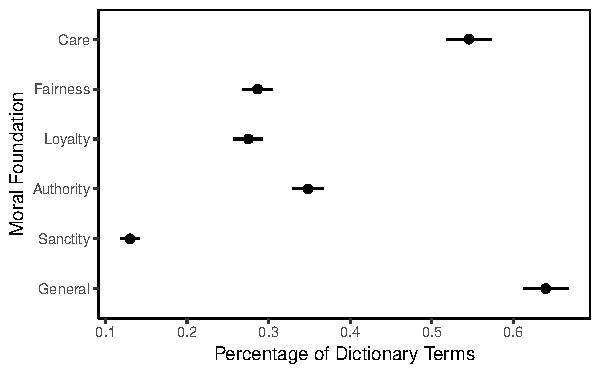
\includegraphics{/data/Dropbox/Uni/Projects/2017/cmv/calc/fig/mft_op_individual.pdf}
\caption[Moral Foundations in Paired Data]{Moral Foundations in Paired Data: Average percentage of dictionary terms relative to the total number of words in each original post starting a discussion (including 95\% confidence intervals). Compared to the figure in the main text, this plot only includes opening statements that are part of the matched pair selection to analyze persuasive arguments.}
\end{figure}


%\clearpage
%\subsection{Distribution of MFT cosine similarity in Paired Data}
%
%\begin{figure}[h]
%\centering
%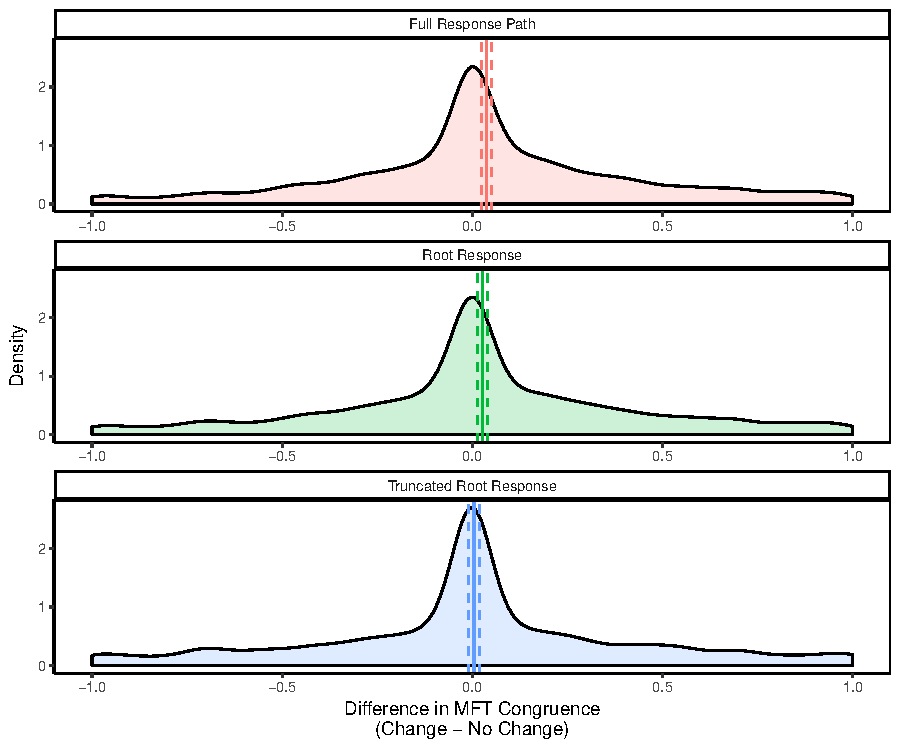
\includegraphics{/data/Dropbox/Uni/Projects/2017/cmv/calc/fig/cosine_density.pdf}
%\caption{Distributions of the difference in MFT cosine similarity.}
%\end{figure}
%
%
%\begin{figure}[h]
%\centering
%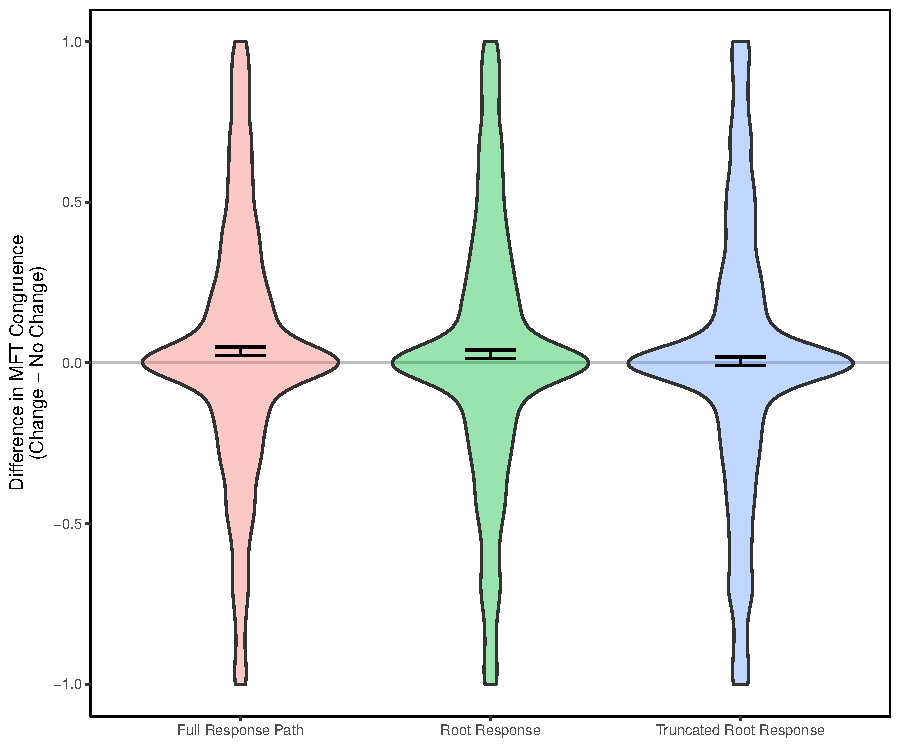
\includegraphics{/data/Dropbox/Uni/Projects/2017/cmv/calc/fig/cosine_violin.pdf}
%\caption{Distributions of the difference in MFT cosine similarity (Violin Plot).}
%\end{figure}

\clearpage
\section{Structural Topic Model Results}\label{app:cmvstm}
%\renewcommand\thefigure{D.\arabic{figure}}
%\renewcommand\thetable{D.\arabic{table}}
%\setcounter{figure}{0}
%\setcounter{table}{0}

\subsection{Original Posts}

\begin{figure}[h]
\centering
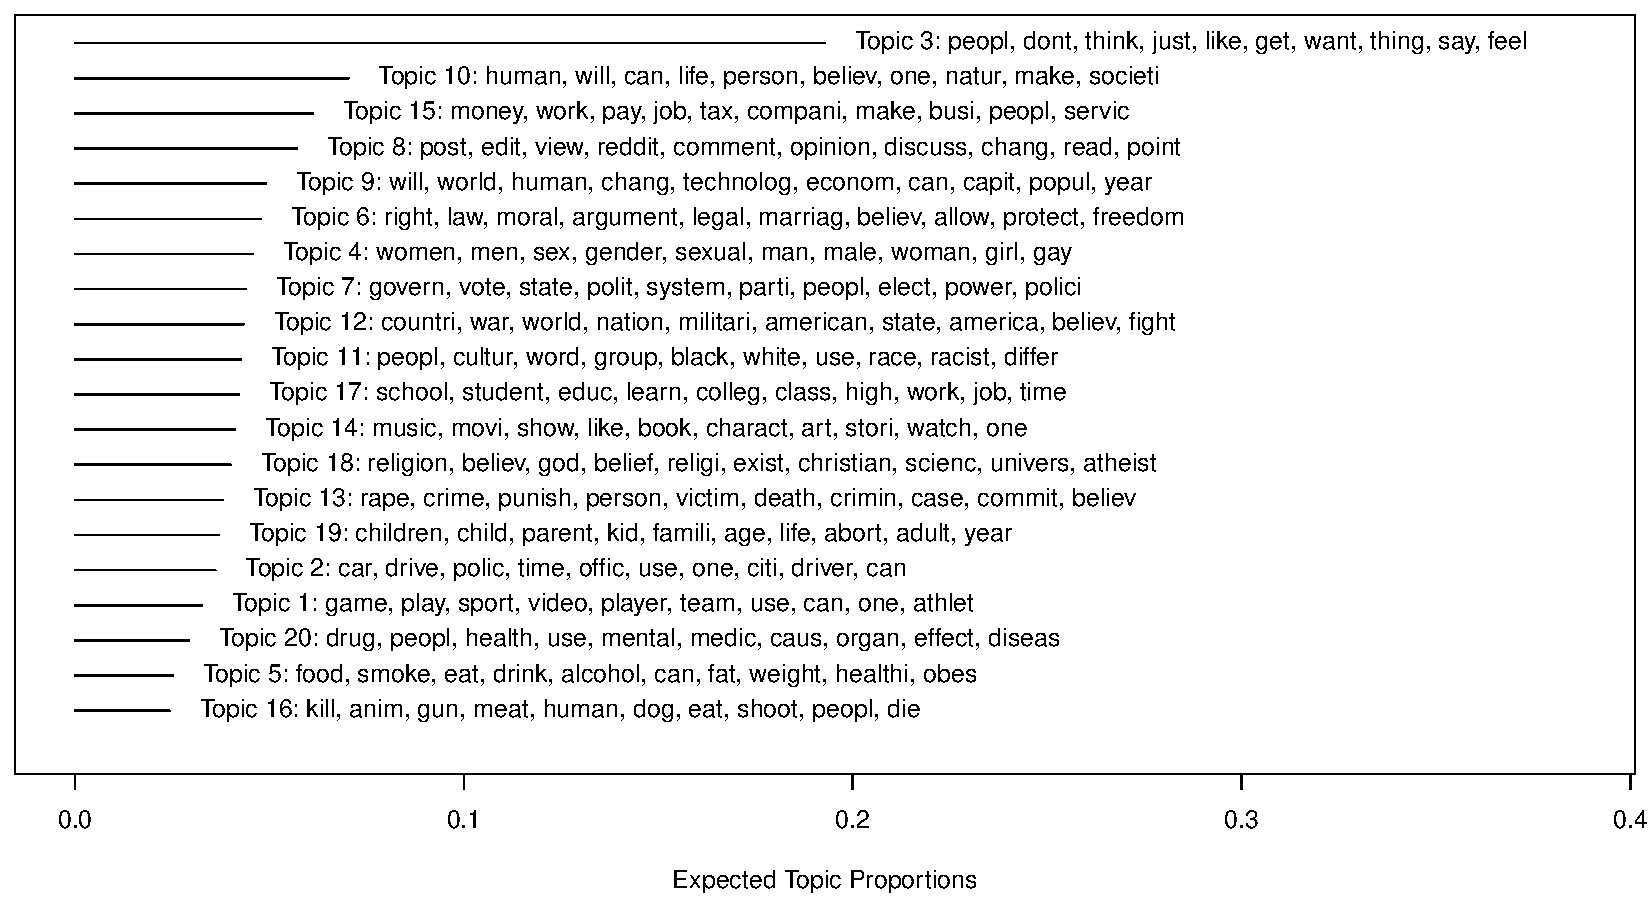
\includegraphics[width=\textwidth]{/data/Dropbox/Uni/Projects/2017/cmv/calc/fig/stm_op_prop.pdf}
\caption[Average topic proportions in opening statements on CMV based on structural topic model]{Average topic proportions in opening statements on \texttt{/r/ChangeMyView/} based on a structural topic model with 20 topics \citep[c.f.,][]{roberts2014structural}. The plot additionally displays the ten most likely terms associated with each respective topic.}
\end{figure}

\begin{figure}[h]
\centering
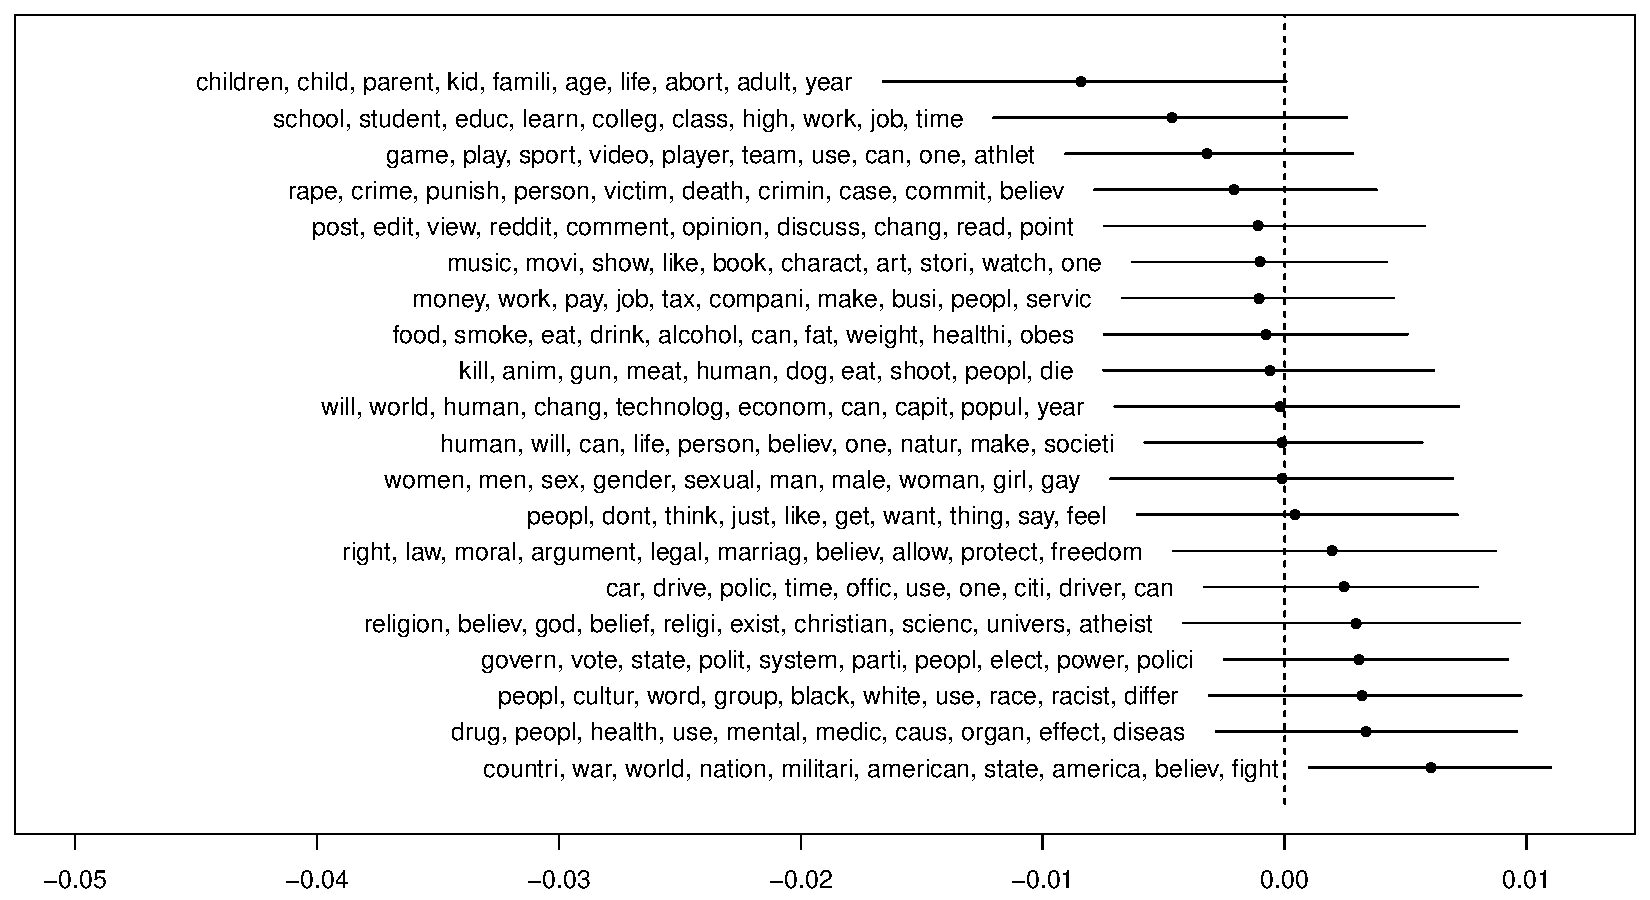
\includegraphics[width=\textwidth]{/data/Dropbox/Uni/Projects/2017/cmv/calc/fig/stm_op_diff.pdf}
\caption[Differences in topic proportions between opening statements on CMV that resulted in opinion change versus not]{Differences in topic proportions between opening statements on \texttt{/r/ChangeMyView/} that resulted in opinion change ($\Delta$ awarded) versus not (including 95\% confidence intervals). Estimates are based on the structural topic model described in the previous figure. Positive values indicate higher topic prevalence among discussions that resulted in opinion change and vice versa. Labels are based on the ten highest probability terms related to the topic.}
\end{figure}

\clearpage
\subsection{Responses Challenging the OP}

\begin{figure}[h]
\centering
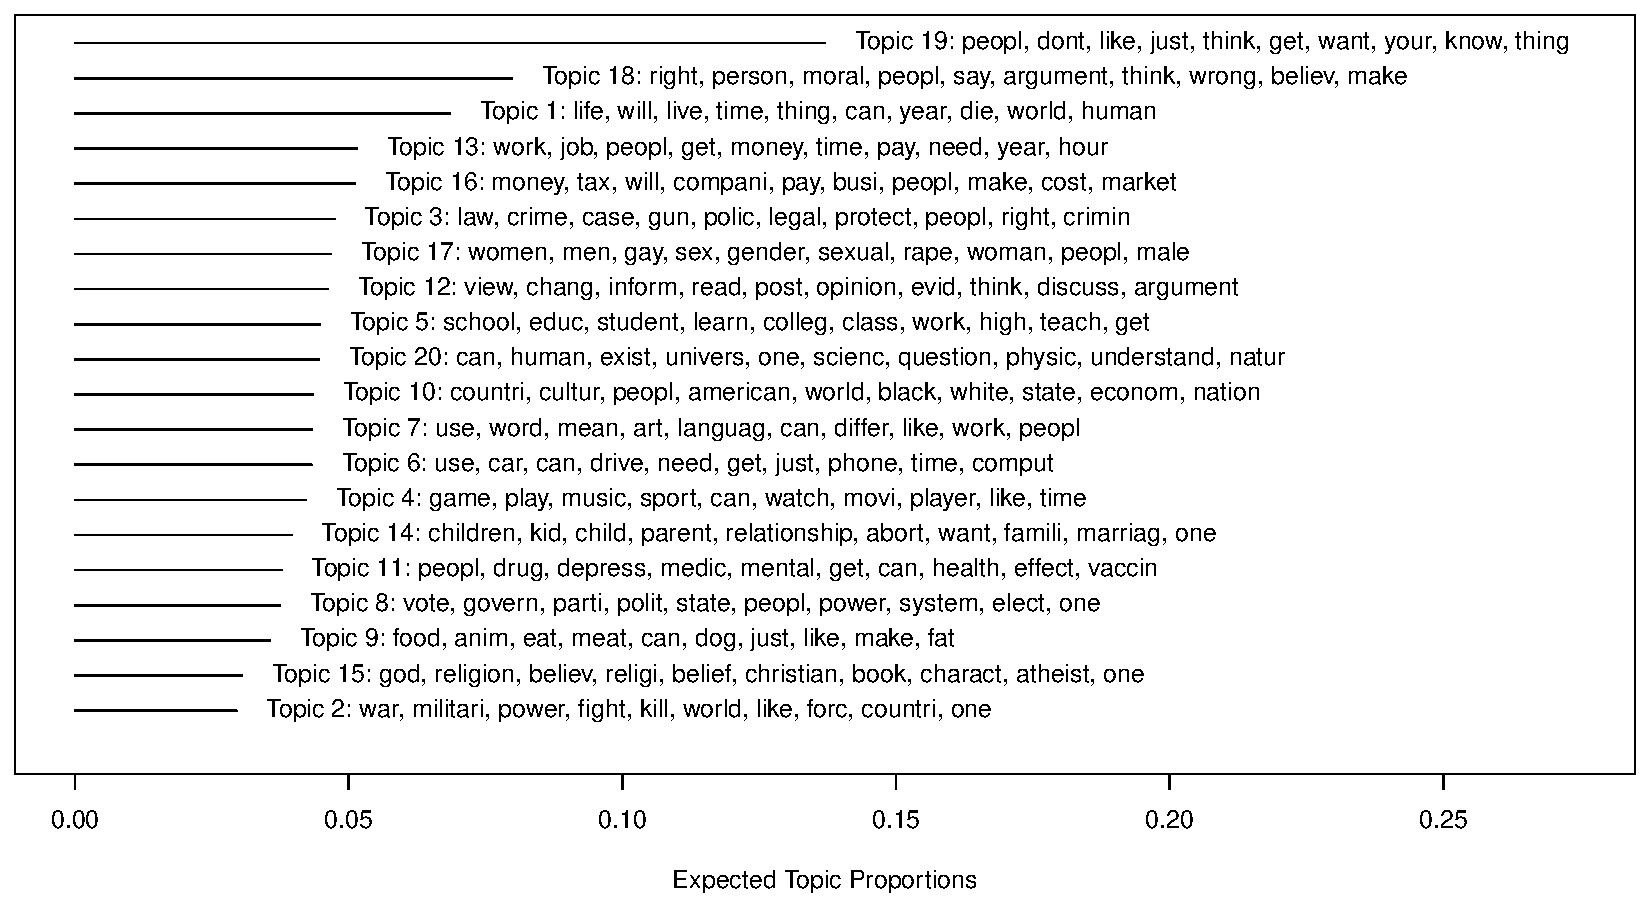
\includegraphics[width=\textwidth]{/data/Dropbox/Uni/Projects/2017/cmv/calc/fig/stm_pair_prop.pdf}
\caption[Average topic proportions in posts challenging the OP on CMV based on structural topic model]{Average topic proportions in posts challenging the OP on \texttt{/r/ChangeMyView/} based on a structural topic model with 20 topics \citep[c.f.,][]{roberts2014structural}. The plot additionally displays the ten most likely terms associated with each respective topic.}
\end{figure}

\begin{figure}[h]
\centering
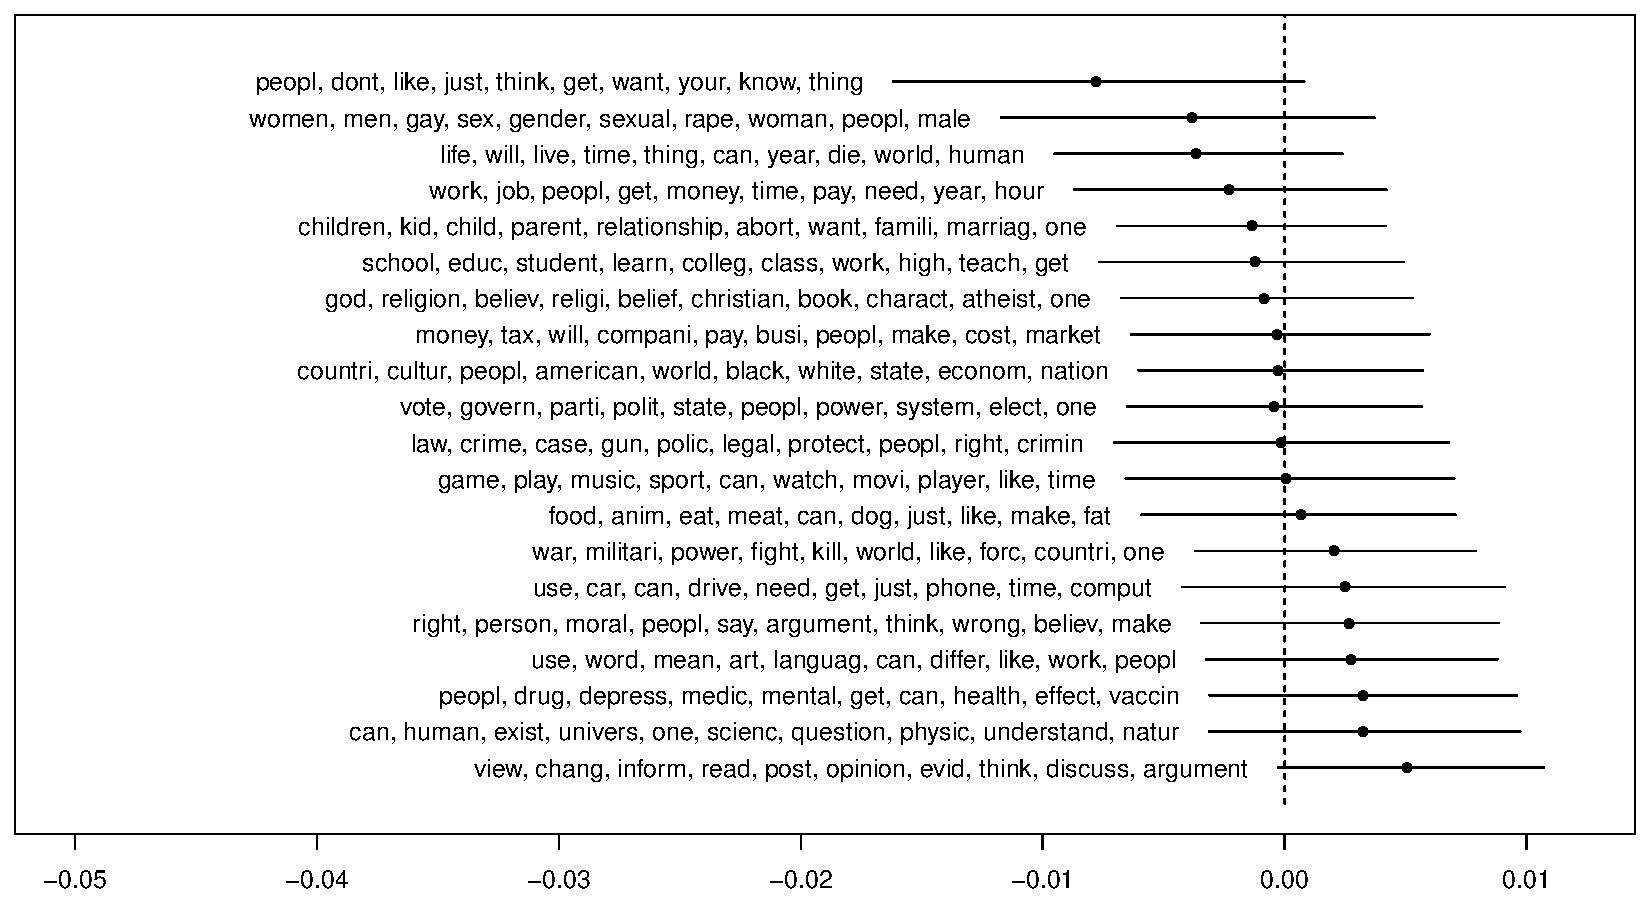
\includegraphics[width=\textwidth]{/data/Dropbox/Uni/Projects/2017/cmv/calc/fig/stm_pair_diff.pdf}
\caption[Differences in topic proportions between persuasive and non-persuasive posts challenging the OP on CMV]{Differences in topic proportions between persuasive and non-persuasive responses challenging the OP (including 95\% confidence intervals). Estimates are based on the structural topic model described in the previous figure. Positive values indicate higher topic prevalence among posts that received a $\Delta$ by the OP and vice versa. Labels are based on the ten highest probability terms related to the topic.}
\end{figure}


\clearpage
\section{Tables of Model Estimates}\label{app:cmvtab}
%\renewcommand\thefigure{E.\arabic{figure}}
%\renewcommand\thetable{E.\arabic{table}}
%\setcounter{figure}{0}
%\setcounter{table}{0}

% latex table generated in R 3.4.2 by xtable 1.8-2 package
% Tue May 15 14:19:34 2018
\begin{table}[ht]
\centering
\caption[Logit models predicting argument persuasiveness as a 
            function of moral word use]{Logit models predicting argument persuasiveness as a 
            function of moral word use (measured via MFT dictionary proportions). 
            Positive coefficients indicate higher probability of changing the OPs'
            mind ($\Delta$ awarded). 
            Standard errors (clustered by discussion thread) in parentheses. Estimates are used for Figure
            \ref{fig:persuasiveness} in the main text.} 
\label{tab:persuasiveness}
\begin{tabular}{lccc}
  \hline
Variable & Full Response Path & Root Response & Truncated Root Response \\ 
  \hline
Care & -0.004 & -0.009 & -0.007 \\ 
   & (0.025) & (0.023) & (0.023) \\ 
  Fairness & -0.029 & -0.024 & -0.032 \\ 
   & (0.036) & (0.033) & (0.031) \\ 
  Loyalty &  0.005 &  0.017 &  0.018 \\ 
   & (0.035) & (0.033) & (0.03) \\ 
  Authority &  0.003 & -0.005 &  0.009 \\ 
   & (0.03) & (0.028) & (0.027) \\ 
  Sanctity & -0.033 & -0.005 & -0.022 \\ 
   & (0.047) & (0.046) & (0.044) \\ 
  General & -0.010 & -0.010 & -0.004 \\ 
   & (0.024) & (0.023) & (0.022) \\ 
  Intercept &  0.018 &  0.015 &  0.009 \\ 
   & (0.024) & (0.023) & (0.022) \\ 
   \hline
N & 6304 & 6304 & 6304 \\ 
  Log-Likelihood & -4369 & -4369 & -4369 \\ 
   \hline
\end{tabular}
\end{table}

% latex table generated in R 3.4.2 by xtable 1.8-2 package
% Tue May 15 14:19:33 2018
\begin{table}[ht]
\centering
\caption[Logit models predicting argument persuasiveness as a 
            function of moral congruence with OPs' opening statements]{Logit models predicting argument persuasiveness as a 
            function of moral congruence with OPs' opening statements (measured via cosine similarity in 
            MFT dictionary results). Positive coefficients indicate higher probability of changing the OPs'
            mind ($\Delta$ awarded). 
            Standard errors (clustered by discussion thread) in parentheses. Estimates are used for Figure
            \ref{fig:cosine} in the main text.} 
\label{tab:cosine}
\begin{tabular}{lccc}
  \hline
Variable & Full Response Path & Root Response & Truncated Root Response \\ 
  \hline
Moral Congruence &  0.290 &  0.188 &  0.019 \\ 
   & (0.056) & (0.056) & (0.054) \\ 
  Intercept & -0.147 & -0.092 & -0.008 \\ 
   & (0.028) & (0.027) & (0.024) \\ 
   \hline
N & 6304 & 6304 & 6304 \\ 
  Log-Likelihood & -4361 & -4366 & -4370 \\ 
   \hline
\end{tabular}
\end{table}
